\documentclass[a4paper,14pt]{extarticle}

\usepackage[T1,T2A]{fontenc}
\usepackage[utf8]{inputenc}
\usepackage[russian]{babel}
\usepackage{geometry}
\usepackage{indentfirst}
\usepackage{graphicx}
\usepackage{url}

\geometry{left=2cm}
\geometry{right=2cm}
\geometry{top=2cm}
\geometry{bottom=2cm}

\linespread{1.5}

\begin{document}

\begin{titlepage}

\begin{center}
  Санкт-Петербургский государственный политехнический университет\\
  Кафедра компьютерных систем и программных технологий
\end{center}

\vspace{13em}

\begin{center}
\textbf{\Large РЕФЕРАТ}

Дисциплина: \textbf{Современные проблемы информатики и вычислительной техники}\\
Тема: \textbf{Анализ подходов и средств для верификации программ.
Использование фреймворков как средств автоматизации}
\end{center}

\vspace{13em}

\begin{flushright}
  Выполнил студент гр. 63501/13 \hspace{8em} А.М. Половцев\\
  Преподаватель \hspace{8em} В.Ф. Мелехин\\
  ``\underline{\hspace{2em}}''\underline{\hspace{8em}} 2013 г.
\end{flushright}

\vspace{\fill}

\begin{center}
  Санкт-Петербург\\
  2013
\end{center}

\end{titlepage}

\tableofcontents

\thispagestyle{empty}

% !TEX root = thesis.tex
%%%%%%%%%%%%%%%%%%%%%%%%%%%%%%%%%%%%%%%%%%%%%%%%%%%%%%%%%%%%%%%%%%%%%%%%%%%%%%%%
\intro
%%%%%%%%%%%%%%%%%%%%%%%%%%%%%%%%%%%%%%%%%%%%%%%%%%%%%%%%%%%%%%%%%%%%%%%%%%%%%%%%

\nomenclature{ПО}{Программное обеспечение}

В данной работе рассматривается подход к автоматизации процесса проведения
анализа и верификации программных систем с целью повышения характеристик
качества.

С развитием вычислительных систем и ростом в них доли программной составляющей,
сложность разрабатываемых программ постоянно возрастает. Также, вследствие
большой конкуренции на рынке программного обеспечения, постоянно снижаются сроки
разработки новых версий ПО. Эти факторы неизбежно ведут к снижению качества
выпускаемых продуктов.

Падение уровня качества является проблемой, особенно если программное
обеспечение задействовано в критически важных сферах человеческой деятельности,
например медицине и космонавтике, так как наличие в них ошибок ведет к большому
материальному ущербу и даже человеческим жертвам. Поэтому задача повышения
качества является одной из самых актуальных в сфере информационных технологий.

Одними из способов повышения качества программ являются статический анализ и
формальные методы, которые часто реализуются в виде инструментальных
средств. При разработке данных средств часто решаются похожие задачи, такие
как:
\begin{itemize}
    \item Построение моделей программы, например, абстрактного синтаксического
    дерева, графа потока управления, графа программных зависимостей и т.д.
    (модели программ рассмотрены в подразделе~\ref{sec:system_models})
    \item Построение различных метрик программного кода
    \item Реинжиниринг программного обеспечения (оптимизация, рефакторинг и т.п.)
    \item Визуализация свойств программной системы
    \item и т.п.
\end{itemize}

Более подробно методы обеспечения качества рассмотрены в
подразделе~\ref{sec:quality_methods}.

Обычно эти задачи решаются вручную каждый раз при создании анализаторов или
проведения верификации программы. В данной работе предлагается способ
автоматизации решения этих задач на основе использования представлений
программы, не зависящих от языка написания ее исходного кода, называемых
метамоделями.

\section{Методы обеспечения качества программного обеспечения}

Существует две основных группы подходов к разработке качественного программного
обеспечения.

\subsection{Подходы, основанные на синтезе ПО} % (fold)

Данная группа основывается на использовании различных формализаций и модельных
представлений во время проектирования архитектуры программной системы. Таким
образом, путем дополнительных усилий на начальном этапе разработки продукта,
можно минимизировать возможность появления ошибок в дальнейших этапах жизненного
цикла.

В данном подходе применяются:

\begin{itemize}
    \item формальные спецификации.
    \item формальные и неформальные описания различных аспектов программной
    системы.
    \item архитектурные шаблоны и стили.
    \item паттерны проектирования.
    \item генераторы шаблонов программ.
    \item генераторы программ.
    \item контрактное программирование.
    \item аннотирование программ.
    \item верификация моделей программ с использованием частичных спецификаций.
    \item использование моделей предметной области для автоматизации
    тестирования программ.
\end{itemize}

\subsection{Подходы, основанные на анализе уже созданного ПО} % (fold)

Данная группа подходов предназначена для повышения качества уже созданного ПО.
Актуальность этой задачи чрезвычайно высока, так как к данному моменту уже
создано огромное количество программных систем, многие из которых имеют проблемы
с уровнем качества, которые проявляются в виде различных ошибок и сбоев.

Предполагается, что уже имеется разработанное программное обеспечение, и
необходимо оценить и повысить его качество. Проверка может заключаться либо в
доказательстве того, что программа соответствует предъявленным функциональным и
нефункциональным требованиям, либо в приведении контрпримеров, показывающих
несоответствие программы этим требованиям.

\newpage
\subsection{Классификация методов обеспечения качества} % (fold)

Обычно выделяют следующие базовые классификации методов обеспечения качества:

\begin{figure}[h!]
    \begin{center}
        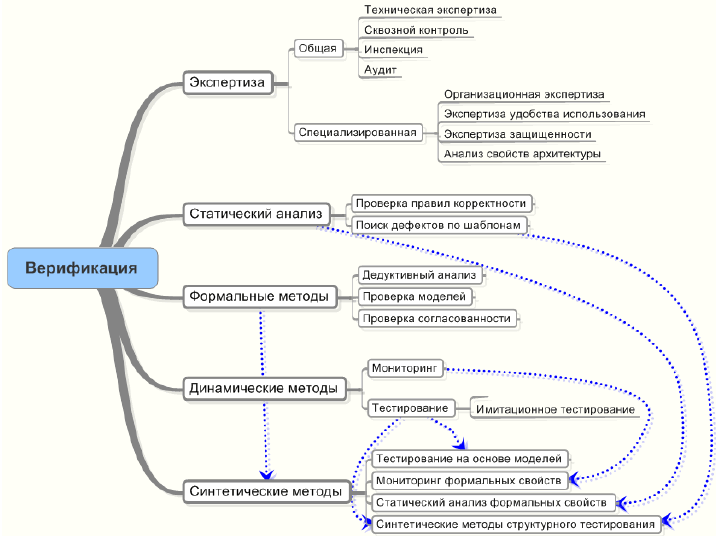
\includegraphics[width=\textwidth]{img/verification_classification.png}
    \end{center}
    \caption{Схема используемой классификации методов верификации}
    \label{fig:figure3}
\end{figure}

\subsubsection{Экспертиза} % (fold)

От других методов верификации экспертизу отличает возможность выполнять ее,
используя только сами артефакты жизненного цикла, а не их модели или результаты
работы, как в формальных и динамических методах. Она позволяет выявлять
практически любые виды ошибок, причем делать это на этапе подготовки
соответствующего артефакта. В то же время она не может быть автоматизирована и
требует активного участия людей.

\subsubsection{Статический анализ} % (fold)

Статический анализ - набор методов, направленный на статический поиск ошибок в
исследуемой программе.

От остальных методов верификации его отделяет то, что статический анализ
позволяет обнаруживать ошибки, вносимые на стадии кодирования. Это связано с
тем, что среди анализируемых артефактов отсутствует спецификация программы, а
это значит, что  анализатор ничего не может знать о том, что делает программа.
Однако, благодаря этому, статический анализ можно полностью автоматизировать.

\subsubsection{Формальные методы} % (fold)

Данные методы использует формальные модели требований, поведения ПО и его
окружения для анализа свойств ПО. К таким методам относятся, например,
дедуктивная верификация, проверка моделей и абстрактная интерпретация.

Эти методы можно применить только к тем свойствам, которые можно выразить в
рамках некоторой математической модели. Построение этой модели не
автоматизируется, а провести анализ таких моделей может лишь специалист. Однако
сама проверка свойств может быть автоматизирована и позволяет находить даже
самые сложные ошибки.

\subsubsection{Динамические методы} % (fold)

Динамические методы используются для анализа и оценки свойств программной
системы по результатам ее реальной работы. Одними из таких методов
являются тестирование и анализ трасс исполнения.

Для применения данных методов необходимо иметь работающую систему (или ее
прототип),  поэтому их нельзя использовать на ранних стадиях разработки. Также
данные методы позволяют найти только те ошибки в ПО, которые проявляются в его
работе.

\subsubsection{Синтетические методы} % (fold)

Данные методы объединяют в себе элементы некоторых способов повышения качества,
описанных выше. Например, существуют динамические методы, использующие элементы
формальных - тестирование на основе моделей (model driven testing) и мониторинг
формальных свойств (runtime verification). Цель таких методов - объединить
преимущества уже используемых подходов.

\section{Модели программных систем} % (fold)
\label{sec:models}

Одной из важнейших составляющих анализа программных систем является построение
модели. Без нее анализатор будет вынужден непосредственно оперировать с исходным
кодом, что влечет за собой усложнение процедур анализа и самого анализатора в
целом.

\subsection{Виды моделей программных систем} % (fold)

В зависимости от способа построения и назначения модели, они могу различаться по
структуре и сложности и обладать различными свойствами. Существуют следующие
виды моделей:

\begin{itemize}
    \item Структурные модели
    \item Поведенческие модели
    \item Гибридные модели
\end{itemize}

Структурные модели во основном используют информацию о синтаксической структуре
анализируемой программы, в то время как поведенческие - информацию о
динамической семантике. Гибридные модели используют оба этих подхода.

\subsubsection{Структурные модели} % (fold)
\begin{enumerate}
    \item Синтаксическое дерево

    Синтаксическое дерево является результатом разбора программы в
    соответствии с формальной грамматикой языка программирования. Вершины
    этого дерева соответствуют нетерминальным символам грамматики, а листья
    - терминальным.

    \item Абстрактное синтаксическое дерево

    Данная модель получается из обычного синтаксического дерева путем
    удаления нетерминальных вершин с одним потомком и замены части
    терминальных вершин их семантическими атрибутами.
\end{enumerate}

\subsubsection{Поведенческие модели} % (fold)
\begin{enumerate}
    \item Граф потока управления

    Граф потока управления представляет потоки управления программы в виде
    ориентированного графа. Вершинами графа являются операторы программы, а дуги
    отображают возможный ход исполнения программы и связывают между собой
    операторы, выполняемые друг за другом.

    \item Граф зависимостей по данным

    Граф зависимостей по данным отображает связь между конструкциями программы,
    зависимыми по используемым данным. Дуги графа соединяют узлы, формирующие
    данные, и узлы, использующие эти данные.

    \item Граф программных зависимостей

    Данная модель объединяет в себе особенности графа потока управления и графа
    зависимости по данным. В графе программных зависимостей присутствуют дуги
    двух типов: информационные дуги отображают зависимости по данным, а
    дуги управления соединяют последовательно выполняемые конструкции.

    \item Представление в виде SSA

    Однократное статическое присваивание (static single assignment) -
    промежуточное представление программы, которое обладает следующими
    свойствами:
        \begin{itemize}
            \item Всем переменным значение может присваиваться только один раз.
            \item Вводится специальный оператор $\phi$-функция, который объединяет
            разные версии локальных переменных.
            \item Все операторы программы представляются в трехоперандной форме.
        \end{itemize}
\end{enumerate}

\subsubsection{Гибридные модели} % (fold)
\begin{enumerate}
    \item Абстрактный семантический граф

    Данная модель является расширением абстрактного синтаксического дерева путем
    добавления дуг, отражающих некоторые семантически свойства программы,
    например, такие дуги могут связывать определение и использование переменной
    или определение функции и ее вызов.
\end{enumerate}

\section{Использование фреймворков для анализа программ} % (fold)

Так как сложность и количество разрабатываемых программных систем постоянно
растет, то для поддержания требуемого уровня качества все чаще начинают
использоваться специализированные инструментальные средства (фреймворки). Данные
средства поддерживают широкий набор инструментов для проведения анализа:

\begin{itemize}
    \item Построение метрик.
    \item Построение моделей программ и применение различных алгоритмов над
    этими моделями.
    \item Интерактивная визуализация процесса анализа.
\end{itemize}

\subsection{Структура фреймворков для анализа программ} % (fold)

Обычно фреймворки строятся по модульному принципу и позволяют пользователю
комбинировать используемые подходы, а также добавлять свои собственные.

На рис~\ref{fig:framework_structure} изображена типичная упрощенная структура
таких фреймворков:

\begin{figure}[h!]
    \begin{center}
        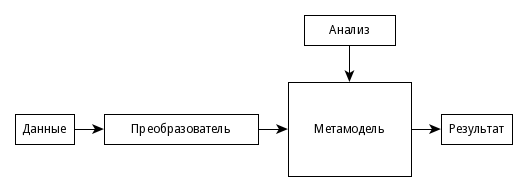
\includegraphics[width=0.7\textwidth]{img/framework_structure.png}
    \end{center}
    \caption{Упрощенная структура фреймворка для анализа программ}
    \label{fig:framework_structure}
\end{figure}

\begin{enumerate}

    \item Входными данными могут являться исходный код анализируемой программы
    или какие-то метаданные, описывающие программную систему.

    \item Преобразователь позволяет привести входные данные к виду, удобному для
    проведения дальнейшего анализа. Эта часть фреймворка является расширяемой -
    пользователь может подключать различные преобразователи для анализа
    соответствующих видов входных данных.

    \item Метамодель является промежуточным представлением анализируемой системы.
    Метамодель должна обладать следующими свойствами:

    \begin{itemize}
        \item Быть независимой от какого-либо языка программирования.
        \item Обладать необходимой полнотой представления для проведения
        различных видов анализа.
        \item Содержать обратную связь с исходными входными данными.
    \end{itemize}

    Метамодели могут поддерживать несколько парадигм программирования,
    однако чаще всего встречаются метамодели, поддерживающие
    только объектно-ориентированное программирование.

    \item После построения метамодели пользователь может использовать ее для
    проведения интересующих его видов анализа. Причем алгоритмы анализа могут
    как входить в состав реализации фреймворка, так и подключаться извне.

    \item Результаты анализа обычно предоставляются в графической или текстовой
    форме.
\end{enumerate}

\subsection{Анализ существующих решений} % (fold)
\subsubsection{SMILE} % (fold)

SMILE - фреймворк для построения метрик программных систем и обладает следующими
характеристиками:

\begin{enumerate}
    \item Независим от языка программирования, на котором написана анализируемая
    система.
    \item Поддерживает большое количество метрик.
    \item Поддерживает анализ различных версий анализируемой системы.
\end{enumerate}

В качестве метамодели SMILE использует представление в виде eCST (enriched
Concrete Syntax Tree), которая представляет собой дерево разбора программы с
добавлением универсальных узлов, что позволяет сделать дерево разбора
независимым от входного языка программирования.

На рис~\ref{fig:smile_arch} изображена архитектура данного фреймворка:

\begin{figure}[h!]
    \begin{center}
        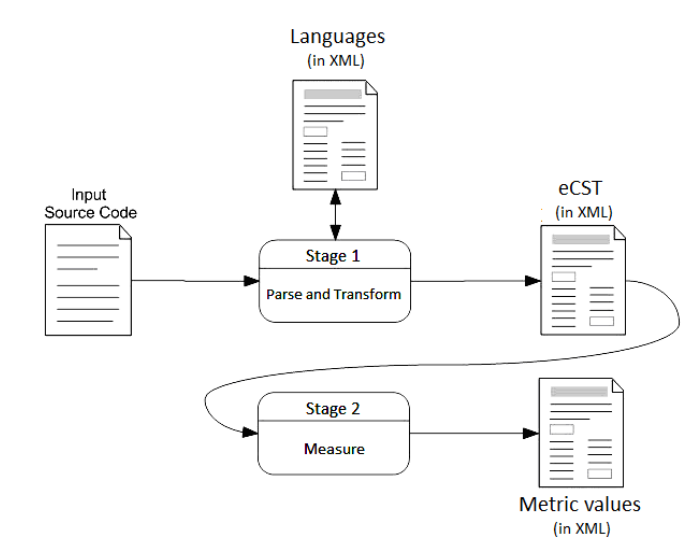
\includegraphics[width=0.6\textwidth]{img/smile_arch.png}
    \end{center}
    \caption{Архитектура фреймворка SMILE}
    \label{fig:smile_arch}
\end{figure}

\newpage
Анализ программы происходит в две фазы:

\begin{enumerate}
    \item Фаза 1
    \begin{itemize}
        \item Определение языка программирования, на котором написана
        анализируемая программа.
        \item Вызов парсера этого языка для построения CST и преобразование в
        eCST.
        \item Вывод результата в формате XML.
    \end{itemize}

    \item Фаза 2
    \begin{itemize}
        \item Считывание eCST из файла.
        \item Подсчет метрик.
        \item Сохранение результата в формате XML.
    \end{itemize}
\end{enumerate}

На данный момент фреймворк находится на стадии разработки и поддерживает
малое количество метрик и языков программирования.

\subsubsection{Moose} % (fold)

Moose является платформой для анализа программ и поддерживает большое количество
различных видов анализа:

\begin{enumerate}
    \item Построение и визуализация метрик.
    \item Обнаружение клонов.
    \item Построение графа зависимостей между пакетами.
    \item Вывод словаря, используемого в проекте.
    \item Поддержка браузеров исходного кода.
\end{enumerate}

Moose использует целое семейство метамоделей под названием FAMIX. Данное
семейство обладает довольно сложной структурой, упрощенная вид которой приведен
на рис~\ref{fig:famix_hierarchy}

\begin{figure}[h!]
     \begin{center}
         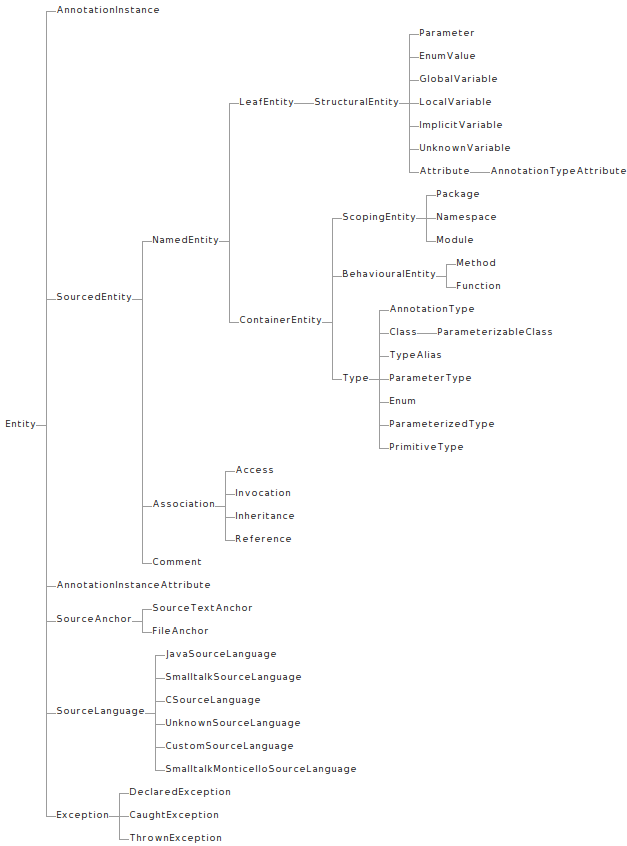
\includegraphics[width=0.9\textwidth]{img/famix_hierarchy.png}
     \end{center}
     \caption{Структура метамоделей семейства FAMIX}
     \label{fig:famix_hierarchy}
 \end{figure}

\newpage
Анализ программы происходит следующим образом:

\begin{enumerate}
    \item Импортирование входных данных. Импортирование может происходить как
    при помощи встроенных средств (Moose поддерживает Smalltalk, XML и MSE),
    так и при помощи сторонних средств.
    \item После импортирования данные приводятся к одной из метамоделей
    семейства FAMIX.
    \item Применение заданных алгоритмов анализа.
\end{enumerate}

Архитектура фреймворка приведена на рис~\ref{fig:moose_architecture}

\begin{figure}[h!]
    \begin{center}
        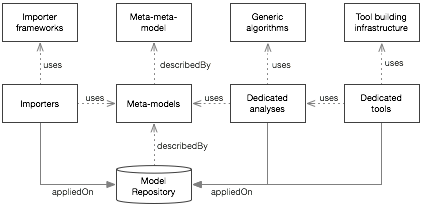
\includegraphics[]{img/moose_architecture.png}
    \end{center}
    \caption{Архитектура фреймворка Moose}
    \label{fig:moose_architecture}
\end{figure}

Разработка Moose активно ведется с 1996 года и на данный момент этот фреймворк
является одним из самых совершенных средств для анализа программ.

\subsubsection{LLVM} % (fold)

LLVM - фреймворк для анализа и трансформации программ, путем предоставления
информации для трансформаций компилятору во время компиляции, линковки и
исполнения.

LLVM использует промежуточное представление, в основе которого лежит
представление в виде SSA. Промежуточное представление является набором
RISC-подобных команд и содержит дополнительную информацию более высокого уровня,
например информацию о типах и графе потока управления.

Фреймворк обладает следующими особенностями:

\begin{enumerate}
    \item Сохранение информации о программе даже во время исполнения и между
    запусками.
    \item Предоставление информации пользователю для профилирования и
    оптимизации.
    \item Промежуточное представление не зависит от языка программирования.
    \item Возможность оптимизации всей системы в целом (после этапа линковки).
\end{enumerate}

Архитектура LLVM приведена на рис~\ref{fig:llvm_arch}

\begin{figure}[h!]
    \begin{center}
        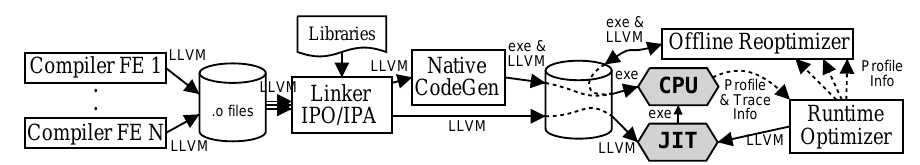
\includegraphics[width=\textwidth]{img/llvm_arch.png}
    \end{center}
    \caption{Архитектура LLVM}
    \label{fig:llvm_arch}
\end{figure}

Front-end компиляторы транслируют исходную программу в промежуточное
представление LLVM, которое затем компонуется LLVM-линкером. На этой стадии
может проводиться межпроцедурный анализ. Получившийся код затем транслируется
в машинный код для целевой платформы.

\section{Постановка задачи} % (fold)

Требуется создать среду для анализа программ, удовлетворяющую следующим
требованиям:

\begin{enumerate}
    \item Предоставлять API на языке Java для проведения анализа, а именно для
    построения метрик и моделей, перечисленных в главе~\ref{sec:models}.
    \item Иметь модульную структуру - позволять подключать пользовательские
    алгоритмы анализа.
    \item Отображать полученные результаты в графическом виде.
\end{enumerate}

После анализа существующих решений было выяснено, что ни один из рассмотренных
фреймворков не удовлетворяет всем перечисленным требованиям, а именно:

\begin{itemize}
    \item SMILE не обладает достаточной зрелостью, чтобы использовать его в
    качестве готового решения.
    \item Moose в основном предназначен для построения метрик программной
    системы и плохо подходит для решения задач верификации.
    \item LLVM предоставляет API только для языков C++ и Ocaml.
\end{itemize}

Исходя из всего вышеперечисленного было принято решение о написании собственного
фреймворка, удовлетворяющим указанным требованиям.

% !TEX root = thesis.tex
%%%%%%%%%%%%%%%%%%%%%%%%%%%%%%%%%%%%%%%%%%%%%%%%%%%%%%%%%%%%%%%%%%%%%%%%%%%%%%%%
\conclusion
%%%%%%%%%%%%%%%%%%%%%%%%%%%%%%%%%%%%%%%%%%%%%%%%%%%%%%%%%%%%%%%%%%%%%%%%%%%%%%%%

В результате выполнения диссертации была разработана инструментальная среда,
позволяющая автоматизировать процедуры анализа и верификации. Для решения данной
задачи был предложен подход с использованием языконезависимой метамодели.

В ходе работы были рассмотрены методы повышения качества и используемые в них
модели ПО (раздел~\ref{chap:analisys}). После обзора способов абстрагирования от
языка программирования для унификации процедур анализа был проведен обзор
существующих средств, использующих метамоделирование. На основе этого обзора
было принято решение о целесообразности разработки собственного средства.

На основе анализа существующих средств и требований, поставленных в
разделе~\ref{chap:task}, была предложена архитектура инструментальной среды,
которая была разделена на три фрагмента - преобразователи, метамодель и
процедуры анализа (раздел~\ref{chap:architeture}). Для каждой составляющей были
предложены варианты реализации.

В разделе~\ref{chap:realisation} была описана реализация разработанной
архитектуры. При реализации использовались приемы и паттерны объектно-
ориентированного программирования, использовался широкий круг библиотек для
решения задач синтаксического разбора, сериализации и визуализации.

На заключительном этапе разработки (раздел~\ref{chap:testing}) было проведено
функциональное тестирование среды, показавшее соответствие разработанной системы
поставленным требованиям.

Разработанную инструментальную среду можно применять для визуализации свойств
программных систем при проведении различных неформальных методов повышения
качества, например, аудита. Функция подсчета метрик позволяет оценивать
характеристики проекта на поздних этапах его жизненного цикла, а визуализацию
графа потока управления можно применять для отладки конкретных процедур
анализируемой системы.

Библиотека с метамоделью может быть использована как промежуточное представление
в формальных методах анализа. Так как метамодель является независимой от языка
программирования, на котором написана анализируемая программная система,
разработанные процедуры анализа можно применять для широкого набора систем.

Дальнейшим развитием проекта является разработка новых видов визуализации,
процедур извлечения новых видов моделей и различных процедур анализа на
основе этих моделей. Также планируется добавление преобразователей для других
популярных языков программирования.


\bibliography{biblio}{}
\bibliographystyle{ugost2008}

\nocite{*}

\end{document}

